\section{Constant Coefficient Equations with Impulses}

\noindent
So far in this chapter, we've considered initial value problems
for the constant coefficient equation
$$
ay''+by'+cy=f(t),
$$
where $f$ is continuous or piecewise continuous on $[0,\infty)$. In
this section we consider initial value problems where $f$
represents a force that's very large for a short time and
zero otherwise. We say that such forces are {\color{blue}\it impulsive\/}.
Impulsive forces occur, for example, when two objects collide. Since
it isn't  feasible to represent such forces as continuous or
piecewise continuous functions, we must construct a different
mathematical model to deal with them.

If $f$ is an integrable function and $f(t)=0$ for $t$ outside of
the interval $[t_0,t_0+h]$, then $\int_{t_0}^{t_0+h} f(t)\,dt$ is
called the {\color{blue}\it total impulse\/} of $f$. We're interested in the
idealized situation where $h$ is so small that the total impulse
can be assumed to be applied instantaneously at $t=t_0$. We say in
this case that $f$ is an {\color{blue}\it impulse function\/}. In particular, we
denote by $\delta(t-t_0)$ the impulse function with total impulse
equal to one, applied at $t=t_0$. (The impulse function $\delta(t)$
obtained by setting $t_0=0$ is  the
\href{https://mathshistory.st-andrews.ac.uk/Biographies/Dirac/}
{\color{blue}\it Dirac
 $\delta$ function\/}.) It must be understood, however, that
$\delta(t-t_0)$ isn't  a function in the standard sense, since our
``definition'' implies that $\delta(t-t_0)=0$ if $t\ne t_0$, while
$$
\int_{t_0}^{t_0} \delta(t-t_0)\,dt=1.
$$
From calculus we know that no function can have these properties;
nevertheless, there's a branch of mathematics known as the
{\color{blue}\it
theory of distributions\/} where  the  definition can be made
rigorous. Since the theory of distributions is beyond the
scope of this book, we'll take an intuitive approach to impulse
functions.

Our first task is to define what we mean by the solution of
the initial value problem
$$
ay''+by'+cy=\delta(t-t_0), \quad  y(0)=0,\quad y'(0)=0,
$$
where $t_0$ is a fixed nonnegative number. The next theorem will
motivate our definition.

\begin{theorem}\color{blue} \label{thmtype:8.7.1}
Suppose $t_0\ge0.$ For each positive number $h,$ let $y_h$ be the
solution of the initial value problem
\begin{equation} \label{eq:8.7.1}
ay_h''+by_h'+cy_h=f_h(t), \quad  y_h(0)=0,\quad y_h'(0)=0,
\end{equation}
where
\begin{equation} \label{eq:8.7.2}
f_h(t)=\left\{\begin{array}{cl} 0,&0\le t<t_0,\\[2\jot]
1/h,&t_0\le t< t_0+h,\\[2\jot]
0,&t\ge t_0+h,\end{array}\right.
\end{equation}
 so  $f_h$ has unit total impulse
equal to the area of the shaded rectangle in Figure~$\ref{figure:8.7.1}$.
Then
\begin{equation} \label{eq:8.7.3}
\lim_{h\to0+}y_h(t)=u(t-t_0)w(t-t_0),
\end{equation}
where
$$
w={\cal L}^{-1}\left(1\over as^2+bs+c\right).
$$
\end{theorem}

\begin{figure}[tbp]
  \centering\color{blue}
  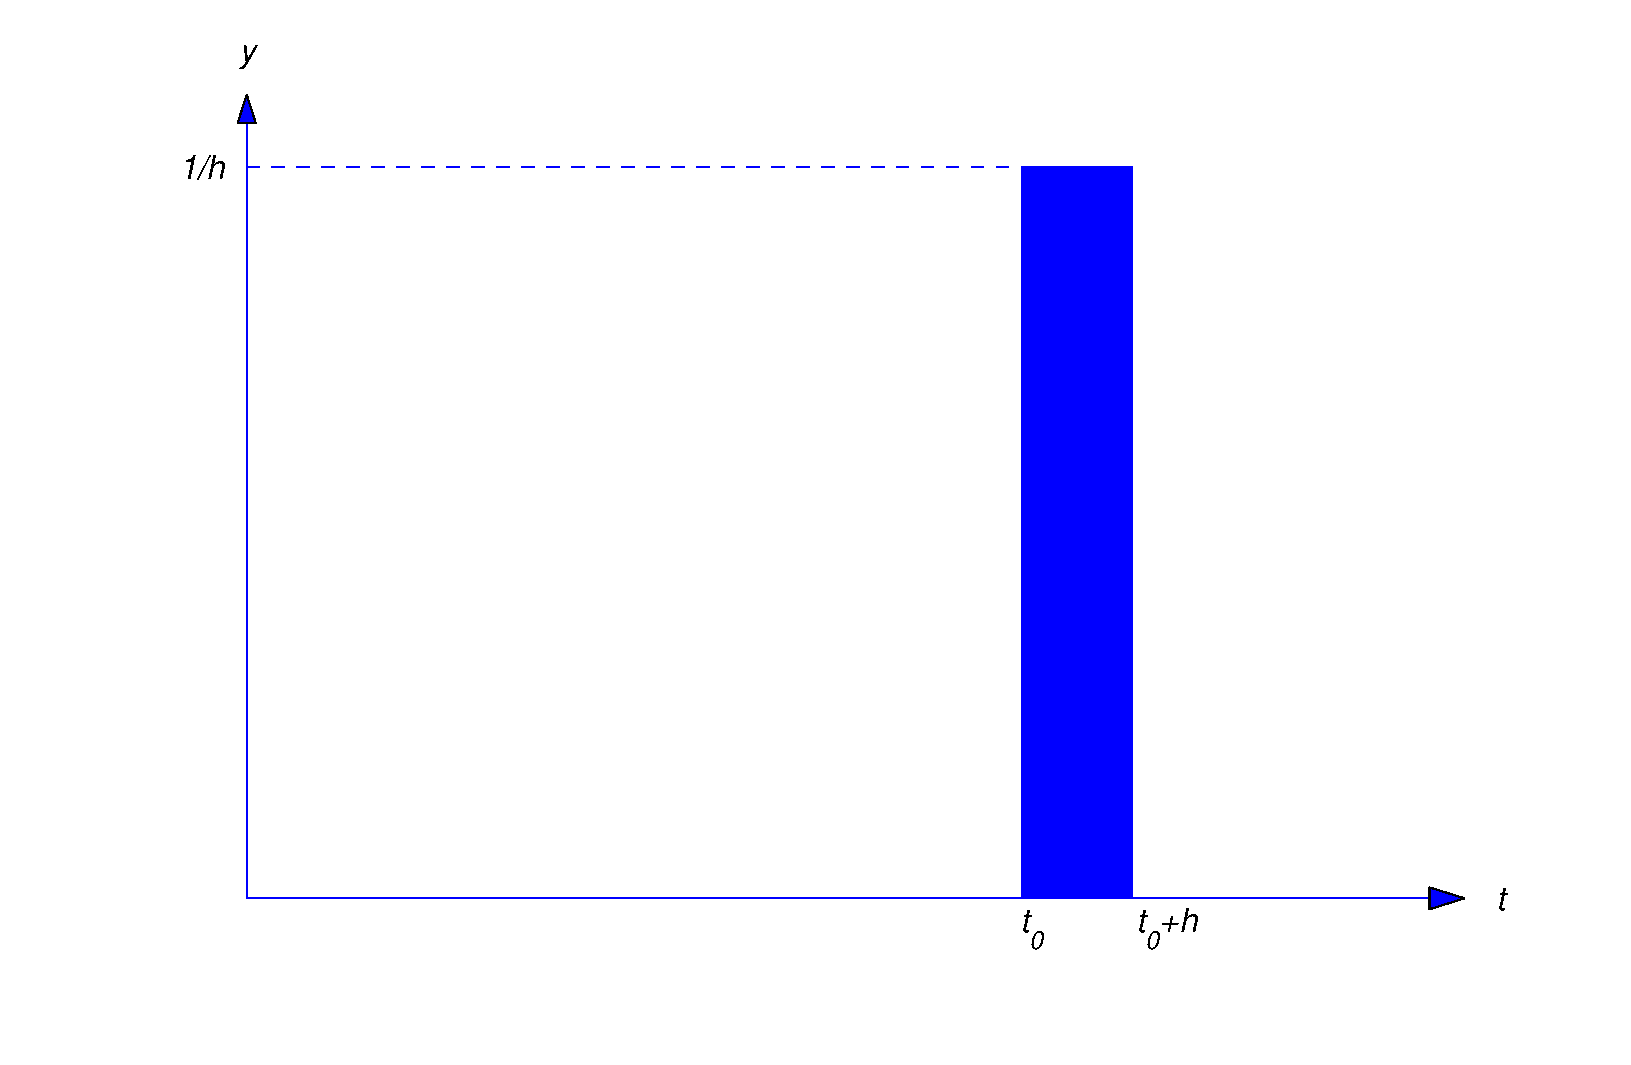
\includegraphics[bb=-78 148 689 643,width=5.67in,height=3.66in,keepaspectratio]{fig080701}
\caption{  $y=f_h(t)$}
  \label{figure:8.7.1}
\end{figure}

\proof
 Taking Laplace transforms in \eqref{eq:8.7.1} yields
$$
(as^2+bs+c)Y_h(s)=F_h(s),
$$
so
$$
Y_h(s)={F_h(s)\over as^2+bs+c}.
$$
The convolution theorem implies that
$$
y_h(t)=\int_0^t w(t-\tau)f_h(\tau)\,d\tau.
$$
Therefore,  \eqref{eq:8.7.2} implies that
\begin{equation} \label{eq:8.7.4}
y_h(t)=\left\{\begin{array}{cl} 0,&0\le t<t_0,\\[2\jot]
\dst{{1\over h}\int_{t_0}^tw(t-\tau)\,d\tau},&t_0\le t\le
t_0+h,\\[2\jot]
\dst{{1\over h
}\int_{t_0}^{t_0+h}w(t-\tau)\,d\tau},&t>t_0+h.\end{array}\right.
\end{equation}
Since $y_h(t)=0$ for all $h$ if $0\le t\le t_0$, it follows that
\begin{equation} \label{eq:8.7.5}
\lim_{h\to0+}y_h(t)=0\mbox{\quad if \quad}0\le t\le t_0.
\end{equation}
We'll now show that
\begin{equation} \label{eq:8.7.6}
\lim_{h\to0+}y_h(t)=w(t-t_0)\mbox{\quad if \quad}t>t_0.
\end{equation}

Suppose   $t$ is fixed and $t>t_0$.
From
\eqref{eq:8.7.4},
\begin{equation} \label{eq:8.7.7}
y_h(t)={1\over h}\int_{t_0}^{t_0+h}w(t-\tau)d\tau\mbox{\quad if \quad}
h<t-t_0.
\end{equation}
Since
\begin{equation} \label{eq:8.7.8}
{1\over h}\int_{t_0}^{t_0+h}d\tau=1,
\end{equation}
we can write
$$
w(t-t_0)={1\over h}w(t-t_0)\int_{t_0}^{t_0+h}\,d\tau=
{1\over h}\int_{t_0}^{t_0+h}w(t-t_0)\,d\tau.
$$
From this and \eqref{eq:8.7.7},
$$
y_h(t)-w(t-t_0)=
{1\over h}\int_{t_0}^{t_0+h}\left(w(t-\tau)-w(t-t_0)\right)\,d\tau.
$$
Therefore
\begin{equation} \label{eq:8.7.9}
|y_h(t)-w(t-t_0)|\le
{1\over h}\int_{t_0}^{t_0+h}|w(t-\tau)-w(t-t_0)|\,d\tau.
\end{equation}
Now let $M_h$ be the maximum value of $|w(t-\tau)-w(t-t_0)|$ as $\tau$
varies over the interval $[t_0,t_0+h]$. (Remember that $t$ and $t_0$
are fixed.) Then \eqref{eq:8.7.8} and \eqref{eq:8.7.9} imply that
\begin{equation} \label{eq:8.7.10}
|y_h(t)-w(t-t_0)|\le
{1\over h}M_h\int_{t_0}^{t_0+h}\,d\tau=M_h.
\end{equation}
But $\lim_{h\to0+}M_h=0$, since $w$ is continuous.
Therefore \eqref{eq:8.7.10} implies \eqref{eq:8.7.6}.
This and \eqref{eq:8.7.5} imply \eqref{eq:8.7.3}. \bbox

Theorem~\ref{thmtype:8.7.1} motivates the next definition.

\begin{definition}\color{blue}\label{thmtype:8.7.2} \rm
If $t_0>0$, then the solution of the initial value problem
\begin{equation} \label{eq:8.7.11}
ay''+by'+cy=\delta(t-t_0), \quad  y(0)=0,\quad y'(0)=0,
\end{equation}
is defined to be
$$
y=u(t-t_0)w(t-t_0),
$$
where
$$
w={\cal L}^{-1}\left(1\over as^2+bs+c\right).
$$
\end{definition}

In physical applications where the input $f$ and the output $y$ of a
device are related by the differential equation
$$
ay''+by'+cy=f(t),
$$
$w$ is called the {\color{blue}\it impulse response\/} of the device. Note
that
$w$ is the solution of the initial value problem
\begin{equation} \label{eq:8.7.12}
aw''+bw'+cw=0, \quad  w(0)=0,\quad  w'(0)=1/a,
\end{equation}
as can be seen by using the Laplace transform to solve this problem.
(Verify.)
On the other hand, we can solve \eqref{eq:8.7.12} by the methods of
Section~5.2 and show that $w$ is defined on
$(-\infty,\infty)$ by
\begin{equation} \label{eq:8.7.13}
w={e^{r_2t}-e^{r_1t}\over a(r_2-r_1)},\quad
w={1\over a}te^{r_1t}, \mbox{\quad or \quad}
w={1\over a\omega}e^{\lambda t}\sin\omega t,
\end{equation}
depending upon whether the polynomial $p(r)=ar^2+br+c$ has distinct
real zeros $r_1$ and $r_2$, a repeated zero $r_1$, or complex
conjugate zeros $\lambda\pm i\omega$. (In most physical applications,
the zeros of the characteristic polynomial have negative real parts,
so $\lim_{t\to\infty}w(t)=0$.) This means that $y=u(t-t_0)w(t-t_0)$ is
defined on $(-\infty,\infty)$ and has the following properties:
$$
y(t)=0,\quad  t<t_0,
$$
$$
ay''+by'+cy=0\mbox{\quad  on \quad }  (-\infty,t_0)\mbox{\quad and
\quad}(t_0,\infty),
$$
and
\begin{equation} \label{eq:8.7.14}
y'_-(t_0)=0, \quad   y'_+(t_0)=1/a
\end{equation}
(remember that $y'_-(t_0)$ and $y'_+(t_0)$ are derivatives from the
right and left, respectively) and $y'(t_0)$ does not exist. Thus, even
though we defined $y=u(t-t_0)w(t-t_0)$ to be the solution of
\eqref{eq:8.7.11},  this function {\color{blue}\it doesn't satisfy\/}
the differential equation in \eqref{eq:8.7.11} {\color{blue}\it at\/} $t_0$, since it
isn't differentiable there;   in fact \eqref{eq:8.7.14} indicates that an
impulse causes a jump discontinuity in velocity. (To see that this is
reasonable, think of what happens when you hit a ball with a bat.)
This means that the initial value problem \eqref{eq:8.7.11} doesn't make
sense if $t_0=0$, since $y'(0)$ doesn't exist in this case. However
$y=u(t)w(t)$ can be defined to be the solution of the modified initial
value problem
$$
ay''+by'+cy=\delta(t), \quad  y(0)=0,\quad y'_-(0)=0,
$$
where the condition on the derivative at $t=0$ has been replaced by a
condition on the derivative from the left.

Figure~\ref{figure:8.7.2} illustrates Theorem~\ref{thmtype:8.7.1} for the
case where the impulse response $w$ is the first expression in
\eqref{eq:8.7.13} and $r_1$ and $r_2$ are distinct and both negative. The
solid curve in the figure is the graph of $w$. The dashed curves are
solutions of \eqref{eq:8.7.1} for various values of $h$. As $h$ decreases
the graph of $y_h$ moves to the left toward the graph of $w$.

\begin{figure}[tbp]
  \centering\color{blue}
  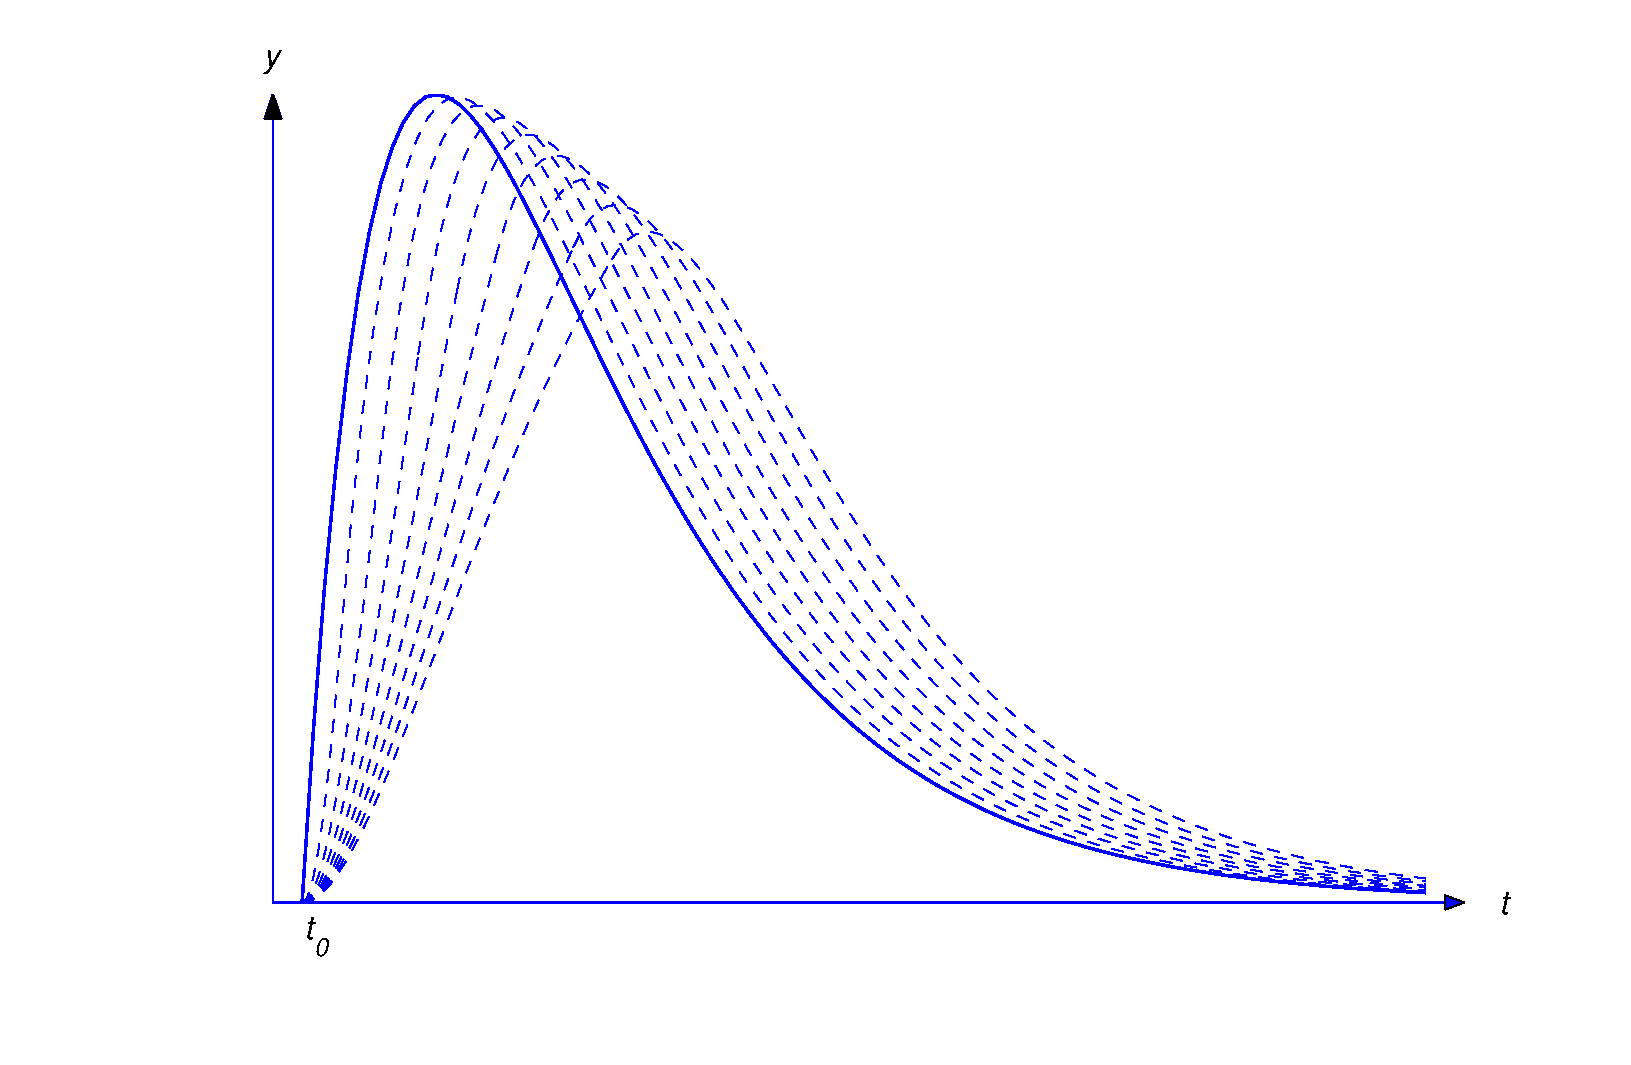
\includegraphics[bb=-78 148 689 643,width=5.67in,height=3.66in,keepaspectratio]{fig080702}
\caption{ An illustration of
Theorem~\ref{thmtype:8.7.1}}
  \label{figure:8.7.2}
\end{figure}

\begin{example}\label{example:8.7.1} \rm  Find the solution of the initial
value problem
\begin{equation} \label{eq:8.7.15}
y''-2y'+y=\delta(t-t_0), \quad  y(0)=0,\quad y'(0)=0,
\end{equation}
where $t_0>0$. Then interpret the solution for the case where $t_0=0$.
\end{example}

\solution
Here
$$
w={\cal L}^{-1}\left(1\over s^2-2s+1\right)={\cal L}^{-1}\left(
1\over(s-1)^2\right)=te^{-t},
$$
so  Definition~\ref{thmtype:8.7.2} yields
$$
y=u(t-t_0)(t-t_0)e^{-(t-t_0)}
$$
as the solution of  \eqref{eq:8.7.15} if $t_0>0$. If $t_0=0$,
then \eqref{eq:8.7.15} doesn't have a solution;     however,
$y=u(t)te^{-t}$
(which we would usually write simply as $y=te^{-t}$) is the solution
of the modified initial value problem
$$
y''-2y'+y=\delta(t), \quad  y(0)=0,\quad y_-'(0)=0.
$$

The graph of $y=u(t-t_0)(t-t_0)e^{-(t-t_0)}$ is shown in
Figure~\ref{figure:8.7.3} \bbox

\begin{figure}[tbp]
  \centering\color{blue}
  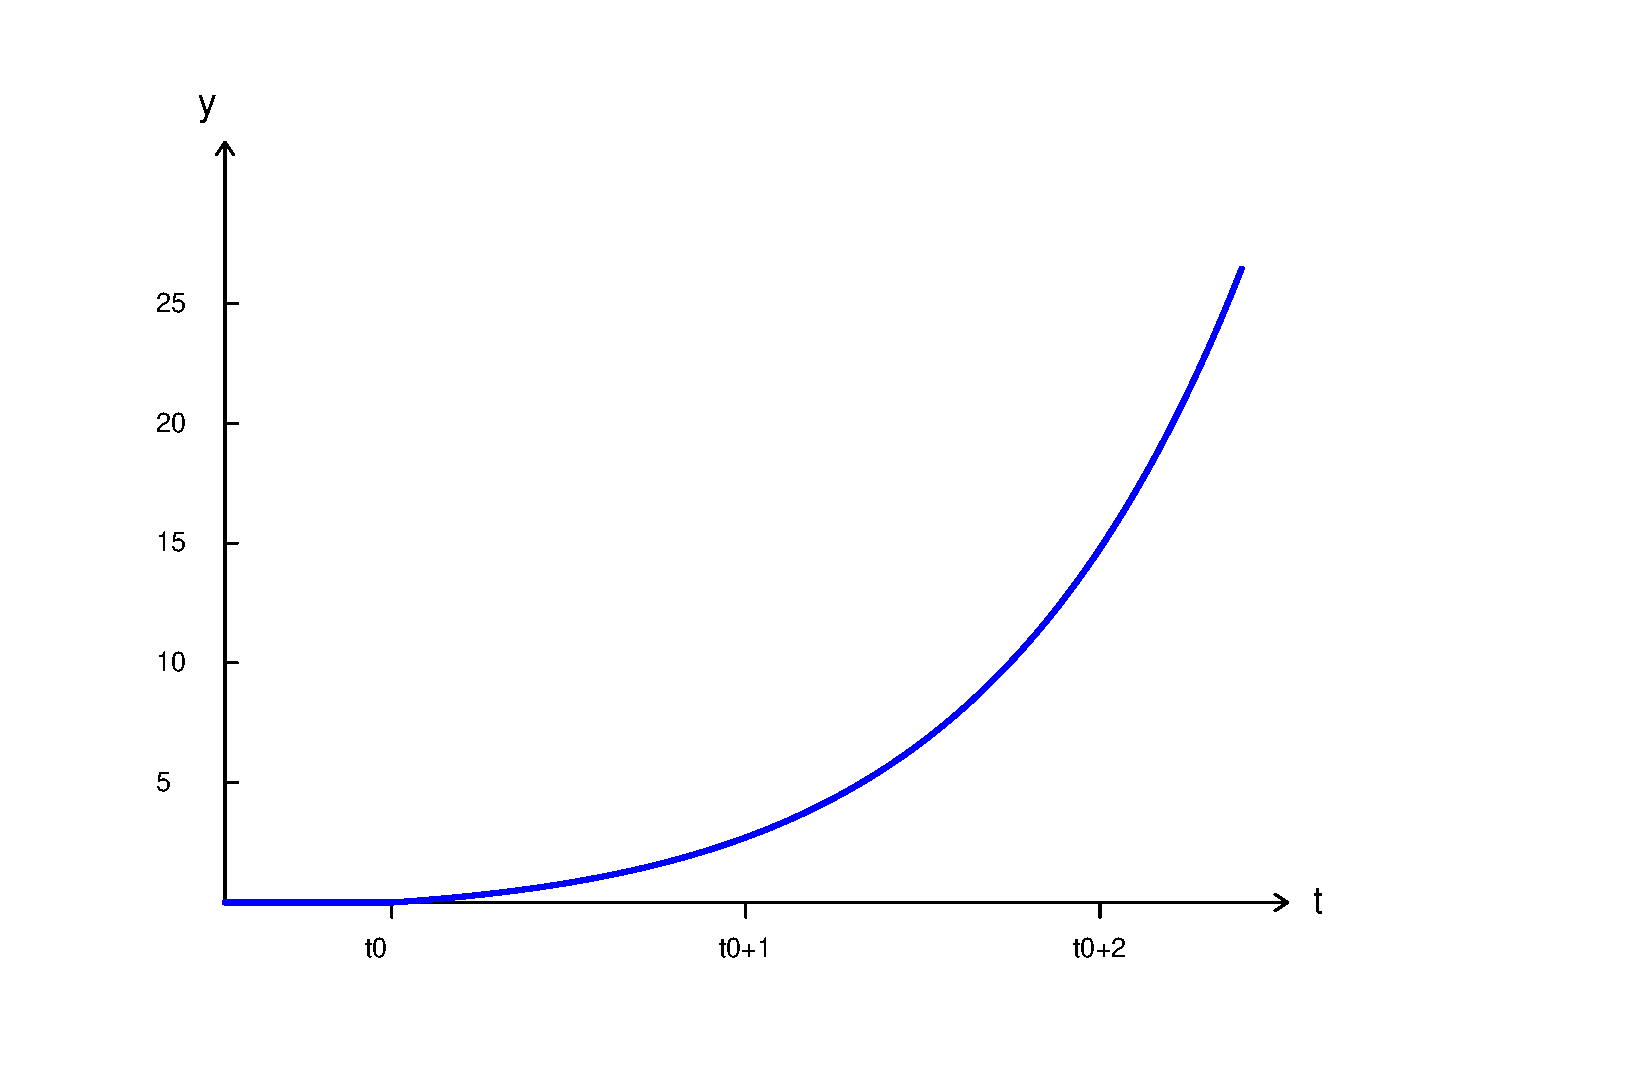
\includegraphics[bb=-78 148 689 643,width=5.67in,height=3.66in,keepaspectratio]{fig080703}
\caption{
$y=u(t-t_0)(t-t_0)e^{-(t-t_0)}$}
  \label{figure:8.7.3}
\end{figure}

Definition~\ref{thmtype:8.7.2} and the principle of superposition
motivate the next definition.

\begin{definition}\color{blue} \label{thmtype:8.7.3} \rm  Suppose
$\alpha$ is a nonzero constant and
$f$ is
piecewise continuous on $[0,\infty)$.
If $t_0>0$, then the solution of  the  initial value problem
$$
ay''+by'+cy=f(t)+\alpha\delta(t-t_0), \quad  y(0)=k_0,\quad y'(0)=k_1
$$
is defined to be
$$
y(t)=\hat y(t)+\alpha u(t-t_0)w(t-t_0),
$$
where $\hat y$  is the solution of
$$
ay''+by'+cy=f(t), \quad  y(0)=k_0,\quad y'(0)=k_1.
$$
This definition also applies if $t_0=0$, provided that the initial
condition $y'(0)=k_1$ is replaced by $y_-'(0)=k_1$.
\end{definition}

\begin{example}\label{example:8.7.2} \rm
Solve the initial value problem
\begin{equation} \label{eq:8.7.16}
y''+6y'+5y=3e^{-2t}+2\delta(t-1),\quad y(0)=-3,\quad y'(0)=2.
\end{equation}
\end{example}

\solution  We leave it to you to show that
the solution of
$$
y''+6y'+5y=3e^{-2t}, \quad    y(0)=-3,\;   y'(0)=2
$$
is
$$
\hat y=-e^{-2t}+{1\over2}e^{-5t}-{5\over2}e^{-t}.
$$
Since
$$
\begin{array}{ccccl}
w(t)&=&{\cal L}^{-1}\left(\dst{1\over s^2+6s+5}\right)&=&
{\cal L}^{-1}\left(\dst{1\over(s+1)(s+5)}\right)\\[2\jot]
&=&\dst{{1\over4}{\cal L}^{-1}\left({1\over s+1}-{1\over s+5}\right)}
&=&\dst{e^{-t}-e^{-5t}\over4},
\end{array}
$$
the solution of  \eqref{eq:8.7.16} is
\begin{equation} \label{eq:8.7.17}
y=-e^{-2t}+{1\over2}e^{-5t}-{5\over2}e^{-t}
+u(t-1){e^{-(t-1)}-e^{-5(t-1)}\over2}
\end{equation}
(Figure~\ref{figure:8.7.4})\bbox.

\begin{figure}[htbp]
\color{blue}
  \begin{minipage}[b]{0.5\linewidth}
    \centering
   \scalebox{.65}{
  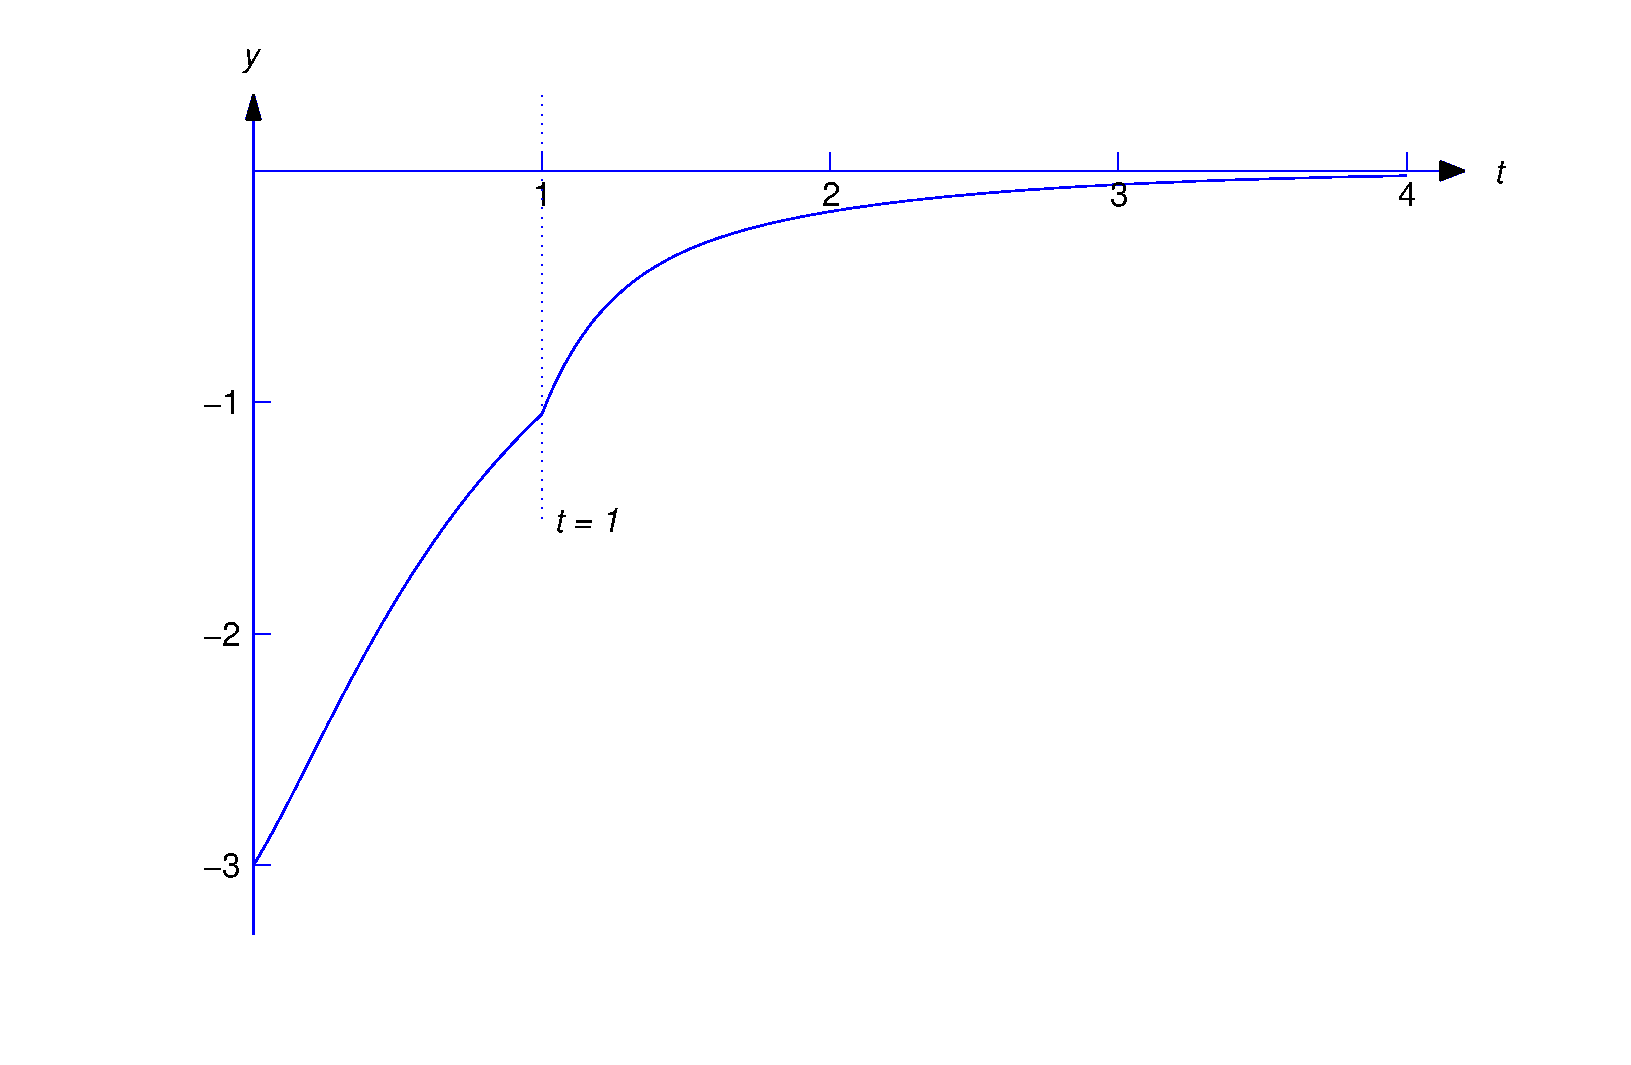
\includegraphics[bb=-78 148 689 643,width=5.67in,height=3.66in,keepaspectratio]{fig080704}}
\caption{ Graph of \eqref{eq:8.7.17}}
  \label{figure:8.7.4}
\end{minipage}
  \begin{minipage}[b]{0.5\linewidth}
    \centering
   \scalebox{.65}{
  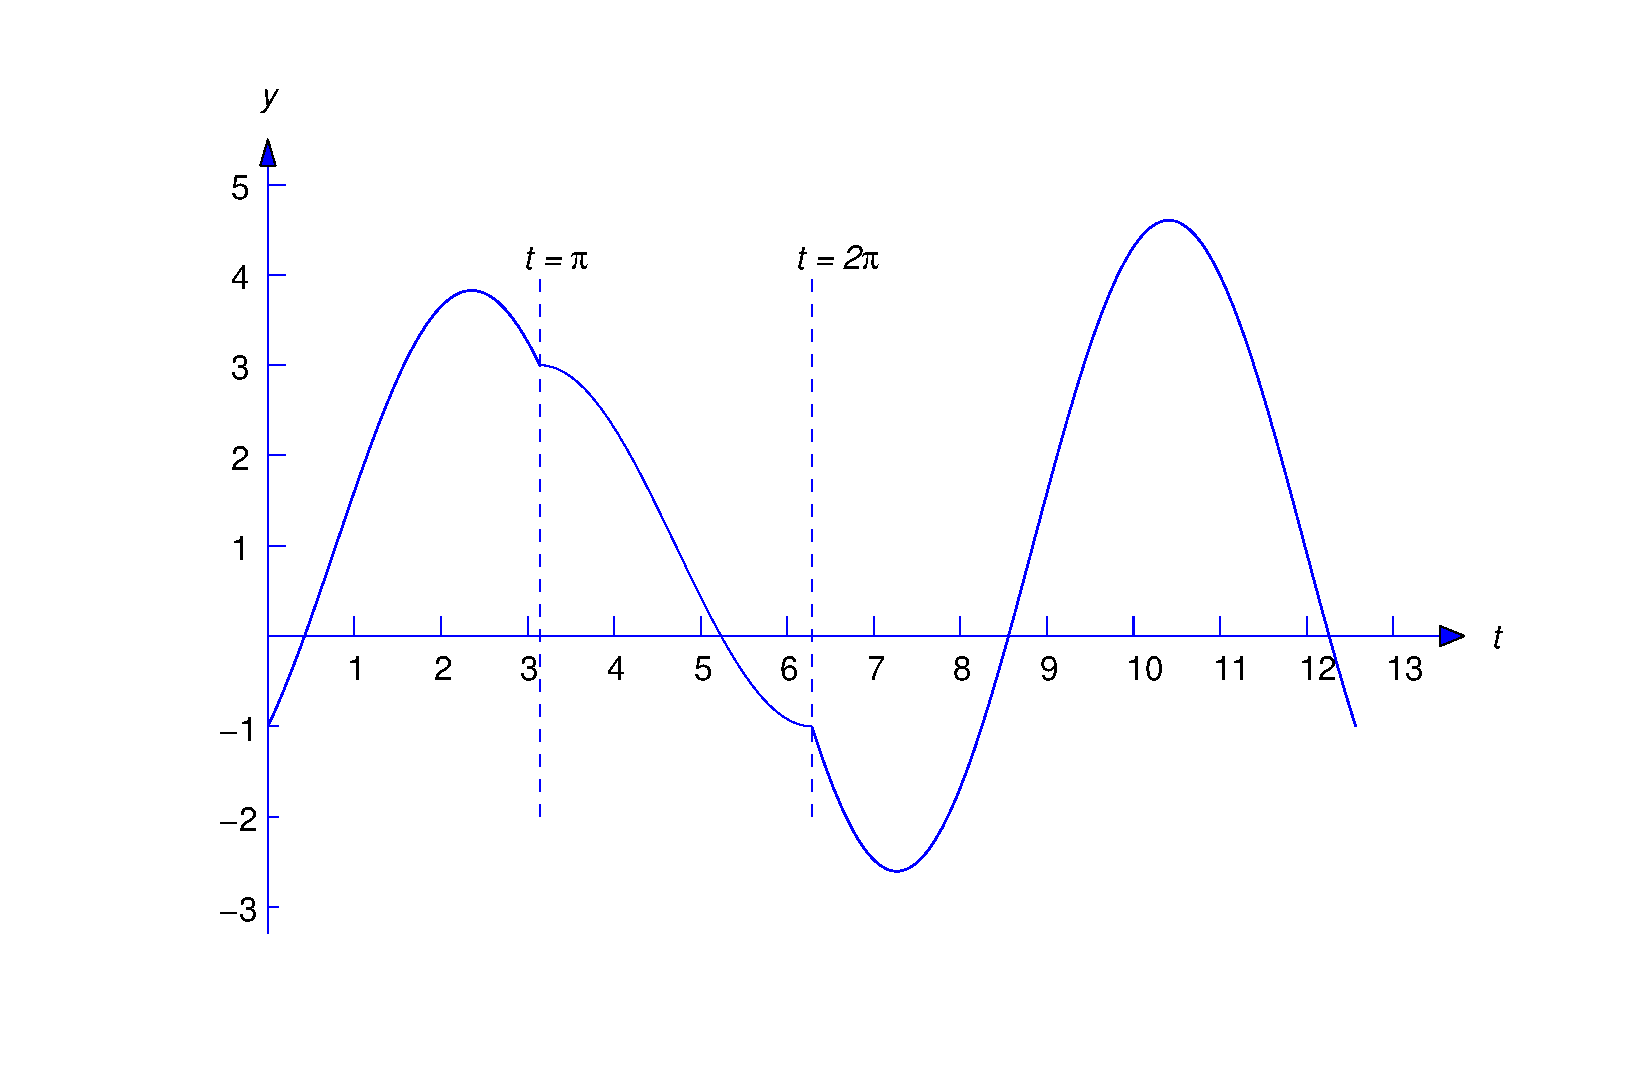
\includegraphics[bb=-78 148 689 643,width=5.67in,height=3.66in,keepaspectratio]{fig080705}}
\caption{ Graph of \eqref{eq:8.7.19}}
  \label{figure:8.7.5}
\end{minipage}
\end{figure}

Definition~\ref{thmtype:8.7.3} can be extended in the obvious way to cover
the case where the forcing function contains more than one impulse.
\begin{example}\label{example:8.7.3} \rm
Solve the  initial value problem
\begin{equation} \label{eq:8.7.18}
y''+y=1+2\delta(t-\pi)-3\delta(t-2\pi), \quad    y(0)=-1,\;   y'(0)=2.
\end{equation}
\end{example}

\solution
We leave it to you to show that
$$
\hat y= 1-2\cos t+2\sin t
$$
is the solution of
$$
y''+y=1, \quad    y(0)=-1,\quad    y'(0)=2.
$$
Since
$$
w={\cal L}^{-1}\left(1\over s^2+1\right)=\sin t,
$$
the solution of  \eqref{eq:8.7.18} is
\begin{eqnarray*}
y&=&1-2\cos t+2\sin t+2u(t-\pi)\sin(t-\pi)-3u(t-2\pi)\sin(t-2\pi)\\
&=&1-2\cos t+2\sin t-2u(t-\pi)\sin t-3u(t-2\pi)\sin t,
\end{eqnarray*}
or
\begin{equation} \label{eq:8.7.19}
y=\left\{\begin{array}{cl} 1-2\cos t+2\sin t,&0\le t<\pi,\\[5pt]
1-2\cos t,&\pi\le t<2\pi,\\[5pt]
1-2\cos t-3\sin t,&t\ge 2\pi\end{array}\right.
\end{equation}
(Figure~\ref{figure:8.7.5}).

\newpage

\exercises
In Exercises~\ref{exer:8.7.1}--\ref{exer:8.7.20} solve the initial value
problem. Where indicated by \CGex, graph the solution.

\begin{exerciselist}
\item\label{exer:8.7.1}
 $y''+3y'+2y=6e^{2t}+2\delta(t-1), \quad  y(0)=2,\quad y'(0)=-6$

\item\label{exer:8.7.2} \CGex
 $y''+y'-2y=-10e^{-t}+5\delta(t-1), \quad  y(0)=7,\quad y'(0)=-9$

\item\label{exer:8.7.3}
 $y''-4y=2e^{-t}+5\delta(t-1), \quad  y(0)=-1,\quad y'(0)=2$

\item\label{exer:8.7.4}  \CGex
 $y''+y=\sin3t+2\delta(t-\pi/2), \quad  y(0)=1,\quad y'(0)=-1$

\item\label{exer:8.7.5}
 $y''+4y=4+\delta(t-3\pi), \quad  y(0)=0,\quad y'(0)=1$

\item\label{exer:8.7.6}
 $y''-y=8+2\delta(t-2), \quad  y(0)=-1,\quad y'(0)=1$

\item\label{exer:8.7.7}
 $y''+y'=e^t+3\delta(t-6), \quad  y(0)=-1,\quad y'(0)=4$

\item\label{exer:8.7.8}
 $y''+4y=8e^{2t}+\delta(t-\pi/2), \quad  y(0)=8,\quad y'(0)=0$

\item\label{exer:8.7.9} \CGex
 $y''+3y'+2y=1+\delta(t-1), \quad  y(0)=1,\quad y'(0)=-1$

\item\label{exer:8.7.10}
 $y''+2y'+y=e^t+2\delta(t-2), \quad  y(0)=-1,\quad y'(0)=2$

\item\label{exer:8.7.11} \CGex
 $y''+4y=\sin t+\delta(t-\pi/2), \quad  y(0)=0,\quad y'(0)=2$

\item\label{exer:8.7.12}
 $y''+2y'+2y=\delta(t-\pi)-3\delta(t-2\pi), \quad  y(0)=-1,\quad y'(0)=2$

\item\label{exer:8.7.13}
$y''+4y'+13y=\delta(t-\pi/6)+2\delta(t-\pi/3), \quad  y(0)=1,\quad y'(0)=2$

\item\label{exer:8.7.14}
$2y''-3y'-2y=1+\delta(t-2), \quad  y(0)=-1,\quad y'(0)=2$

\item\label{exer:8.7.15}
$4y''-4y'+5y=4\sin t-4\cos
t+\delta(t-\pi/2)-\delta(t-\pi), \quad  y(0)=1,\quad y'(0)=1$

\item\label{exer:8.7.16}
$y''+y=\cos2t+2\delta(t-\pi/2)-3\delta(t-\pi), \quad  y(0)=0,\quad y'(0)=-1$

\item\label{exer:8.7.17} \CGex
$y''-y=4e^{-t}-5\delta(t-1)+3\delta(t-2), \quad  y(0)=0,\quad y'(0)=0$

\item\label{exer:8.7.18}
$y''+2y'+y=e^t-\delta(t-1)+2\delta(t-2), \quad  y(0)=0,\quad y'(0)=-1$

\item\label{exer:8.7.19}
$y''+y=f(t)+\delta(t-2\pi), \quad  y(0)=0,\quad y'(0)=1$, \text{and}

$f(t)=\dst{\left\{\begin{array}{cl}
\sin2t,&0\le t<\pi,\\[5pt]0,&t\ge \pi.\end{array}\right.}$

\item\label{exer:8.7.20}
$y''+4y=f(t)+\delta(t-\pi)-3\delta(t-3\pi/2), \quad  y(0)=1,\quad
y'(0)=-1$, \text {and}

$f(t)=\dst{\left\{\begin{array}{cl}1,&0\le t<\pi/2,\\[5pt]2,&t\ge
\pi/2\end{array}\right.}$

\item\label{exer:8.7.21}
$y''+y=\delta(t), \quad  y(0)=1,\quad y_-'(0)=-2$

\item\label{exer:8.7.22}
$y''-4y=3\delta(t), \quad  y(0)=-1,\quad y_-'(0)=7$

\item\label{exer:8.7.23}
$y''+3y'+2y=-5\delta(t), \quad  y(0)=0,\quad y_-'(0)=0$

\item\label{exer:8.7.24}
$y''+4y'+4y=-\delta(t), \quad  y(0)=1,\quad y_-'(0)=5$

\item\label{exer:8.7.25}
$4y''+4y'+y=3\delta(t), \quad  y(0)=1,\quad y_-'(0)=-6$

\exercisetext{
In Exercises~\ref{exer:8.7.26}-\ref{exer:8.7.28}, solve the initial value
problem
$$
ay_h''+by_h'+cy_h=
\left\{\begin{array}{cl} 0,&0\le t<t_0,\\[2\jot]
1/h,&t_0\le t< t_0+h,\\[2\jot]
0,&t\ge t_0+h,\end{array}\right.
\quad y_h(0)=0,\quad y_h'(0)=0,
$$
where $t_0>0$ and $h>0$. Then find
$$
w={\cal L}^{-1}\left(1\over as^2+bs+c\right)
$$
and verify Theorem~\ref{thmtype:8.7.1} by graphing $w$ and $y_h$
on the same axes, for small positive values of $h$.}

\item\label{exer:8.7.26} \Lex
$y''+2y'+2y=f_h(t), \quad  y(0)=0,\quad y'(0)=0$

\item\label{exer:8.7.27} \Lex
$y''+2y'+y=f_h(t), \quad  y(0)=0,\quad y'(0)=0$

\item\label{exer:8.7.28} \Lex
$y''+3y'+2y=f_h(t), \quad  y(0)=0,\quad y'(0)=0$

\item\label{exer:8.7.29}

Recall from Section~6.2 that the displacement of
an
object of mass $m$ in a spring--mass system in free damped oscillation is
$$
my''+cy'+ky=0, \quad  y(0)=y_0,\quad y'(0)=v_0,
$$
and that $y$ can be written as
$$
y=Re^{-ct/2m}\cos(\omega_1t-\phi)
$$
if the motion is underdamped. Suppose $y(\tau)=0$.
Find the impulse that would have to be applied to the object at $t=\tau$
 to put it in equilibrium.

\item\label{exer:8.7.30} Solve the initial value problem. Find a formula that
does not involve step functions and represents $y$  on each subinterval of
$[0,\infty)$  on which the forcing function is zero.

{\bf (a)} $\dst{y''-y=\sum_{k=1}^\infty\delta(t-k), \quad  y(0)=0,\quad y'(0)=1}$

{\bf (b)}
$\dst{y''+y=\sum_{k=1}^\infty\delta(t-2k\pi), \quad  y(0)=0,\quad y'(0)=1}$

{\bf (c)}
$\dst{y''-3y'+2y=\sum_{k=1}^\infty\delta(t-k), \quad  y(0)=0,\quad y'(0)=1}$

{\bf (d)}
$\dst{y''+y=\sum_{k=1}^\infty\delta(t-k\pi), \quad  y(0)=0,\quad y'(0)=0}$

\end{exerciselist}
